\section{Causal Impact: Definitions}\label{sec:causal_impact}

Explanation and causal attribution seek to connect a potentially causal \textit{event} $X=x$ to an outcome event $Y=y$.\footnote{This is quite different from type-level causal queries, where one is interested in some group-level attribution, as when one estimates average treatment effect or conditional average treatment effect.}
% To measure the strength of causation, we (i) intervene to change $X$ and measure the extent to which this changes $Y$ (call this a \emph{necessity intervention}), and (ii) intervene on $X$ to have the actual value and measure the extent to which this ensures $Y=y$ (call this a \emph{sufficiency intervention}), while (iii) preserving context-sensitivity, and (iv) allowing for some variation in which parts of the contexts are fixed and in what combinations the cause candidates are intervened on, to account for interactions.
% Moreover, (v) to search for causes, we also need to perform a search through potential sets of causes.
In this section, we present a formal development. To ground it, we return to Example~\ref{ex:obcb_stochastic} and
 use Alice and Bob as running illustrations throughout this section. Both are rejected for a loan; the question is
 which of their attributes (\varname{gender} and \varname{credit}) was causally responsible for each rejection,
 and to what degree. While the example is discrete, the machinery applies to continuous and mixed-type variables;
  a continuous illustration is given in Sections~\ref{sec:signal} and~\ref{sub:synthetic}.

\paragraph{Roadmap of this section.}
We state seven \emph{desiderata} that any responsibility attribution for Alice and Bob should satisfy, giving the formal construction an explicit target. We introduce the probabilistic
structural causal model (PSCM) and interventions, the substrate on which everything
else rests, and then the two distributions \ourapproach offers to the user: the
variable selection distribution $\Gamma$ over suspect/witness pairs and the
alternative-value distribution $\Delta$ over counterfactual cause settings. We combine
these into the joint necessity-sufficiency measure $P_k^{s,n}$ and the user-chosen
causal impact function $ci$ whose expectation is the \ourapproach score, showing how
the choice of $ci$ generalises the framework from binary to continuous outcomes.
Finally we compute the score on the OBCB example, verify that all seven desiderata
hold, and contrast \ourapproach's necessity/sufficiency decomposition with Pearl's
PN/PS/PNS.

Let $R(V \rightsquigarrow \varname{loan} \mid \text{person})$ denote the causal responsibility of variable $V$
for the loan outcome at the individual level ($R$ is a placeholder for any attribution score and
should not be identified with a specific formal quantity; \ourapproach interprets $R$ as the
PCI score $\mathrm{PCI}_{X_k}$ of Definition~\ref{def:causalimpact}, but the desiderata are
method-agnostic). Here $V$ ranges over the candidate variables; in the general development
it is the variable of interest $X_k$.
Attribution methods may produce signed values; the desiderata are stated in terms of absolute
magnitudes $|R(\cdot)|$, allowing for directionality:
\label{desid}
\begin{align*}
\textbf{D-A1} \quad & |R(\varname{gender} \rightsquigarrow \varname{loan} \mid \text{Alice})| > 0 \\[2pt]
\textbf{D-A2} \quad & |R(\varname{credit} \rightsquigarrow \varname{loan} \mid \text{Alice})| > 0 \\[2pt]
\textbf{D-A-rank} \quad & |R(\varname{gender} \rightsquigarrow \varname{loan} \mid \text{Alice})| > |R(\varname{credit} \rightsquigarrow \varname{loan} \mid \text{Alice})| \\[6pt]
\textbf{D-B1} \quad & |R(\varname{gender} \rightsquigarrow \varname{loan} \mid \text{Bob})| > 0 \\[2pt]
\textbf{D-B2} \quad & |R(\varname{credit} \rightsquigarrow \varname{loan} \mid \text{Bob})| > 0 \\[2pt]
\textbf{D-B-rank} \quad & |R(\varname{credit} \rightsquigarrow \varname{loan} \mid \text{Bob})| > |R(\varname{gender} \rightsquigarrow \varname{loan} \mid \text{Bob})| \\[6pt]
\textbf{D-comp} \quad & |R(\varname{gender} \rightsquigarrow \varname{loan} \mid \text{Alice})| > |R(\varname{gender} \rightsquigarrow \varname{loan} \mid \text{Bob})|
\end{align*}

\noindent \textbf{D-A1} and \textbf{D-A2} both require non-zero attribution for Alice because two
distinct causal routes were available. Gender filtered her out at the checking stage. Credit is not
causally inert either: the check is only \emph{probabilistic} (women are still checked with positive
probability, $\gamma_F=0.2$ in the model below), so conditioning on Alice's denial leaves nonzero
probability that she was in fact checked, in which case her bad credit was the operative cause. The
broader principle is a graded ordering of three roles. An \emph{active} cause, on the path that actually
produced the outcome, carries the most responsibility. A \emph{preempted} cause is not discarded but
retains a \emph{residual} share, strictly positive yet strictly below the active cause (exactly what
\textbf{D-A-rank} demands), here governed by the probability that the preemption fails to fire,
leaving the credit route live. An \emph{irrelevant} variable, with no active path to the outcome under
any context, receives the least of all, approaching zero. This is a deliberate departure from the binary
Halpern--Pearl/Beckers treatment of preemption, which collapses the first two roles by zeroing a fully
preempted cause. \textbf{D-A-rank} is the substantive constraint: because Alice never underwent a
credit evaluation, gender's causal role is immediate, whereas credit's is purely
hypothetical. A method that ranks credit above gender for Alice is misattributing the cause of her
rejection.

For Bob, \textbf{D-B2} reflects that the credit check occurred and directly produced the rejection:
the causal chain $\varname{credit} \to \varname{check\text{-}failed} \to \varname{loan}$ was
activated. \textbf{D-B1} requires strictly positive attribution for \varname{gender}: being male
gave Bob a $90\%$ probability of being checked, so gender opened the evaluation that rejected him.
This indirect causal role is non-zero; a method returning exactly zero fails to capture it.
\textbf{D-B-rank} corresponds to the intuition that credit is the proximate cause.
\textbf{D-comp} captures the cross-individual asymmetry that is hardest for naive methods to
express: gender is more causally responsible for Alice's rejection than for Bob's, because for
Alice \varname{gender}=female was sufficient on its own to produce the rejection (no
evaluation took place, so credit was never a factor), while for Bob \varname{gender}=male
merely opened the evaluation that \varname{credit}=bad then caused.
We will verify at the end of this section that \ourapproach satisfies all seven desiderata,
while PN, PS, PNS fail some of them. Later, we will also revisit this example and its
 desiderata in the context of SHAP and Causal SHAP (Section~\ref{sec:shap_examples}).

We work within the context of probabilistic structural causal models \citep{causalityPearl}.
\begin{definition}[Probabilistic Structural Causal Model (PSCM)]
A probabilistic structural causal model is a tuple
\[
M = \langle \mathbf{U}, \mathbf{V}, \mathbf{F}, P_{\mathbf{U}} \rangle,
\]
where \(\mathbf{V} = \{V_1,\dots,V_n\}\) is a finite set of endogenous variables,
\(\mathbf{U} = \{U_1,\dots,U_n\}\) is a set of exogenous variables,
and \(\mathbf{F} = \{f_1,\dots,f_n\}\) is a set of structural assignments
\[
V_i := f_i(\mathbf{Pa}_i, U_i), \qquad i = 1,\dots,n,
\]
with \(\mathbf{Pa}_i \subseteq \mathbf{V}\setminus\{V_i\}\) denoting the parents of \(V_i\).
The distribution \(P_{\mathbf{U}}\) is a probability measure on $\dom(\mathbf{U})$,
and the assignments in \(\mathbf{F}\) are assumed to be acyclic and to have a unique solution for \(\mathbf{V}\) given \(\mathbf{U}\).\footnote{Working within the PSCM framework commits the practitioner to fully specified structural assignments $\mathbf{F}$ and an exogenous distribution $P_{\mathbf{U}}$, analogous to how Bayesian inference requires a likelihood and a prior. This is precisely what enables \ourapproach to yield individual-level counterfactual attributions rather than population-level bounds, and once $\mathbf{F}$ and $P_{\mathbf{U}}$ are specified, sampling from $P_{\mathbf{U}}$ is a routine probabilistic inference operation.}
\end{definition}

\medskip\noindent A PSCM encodes which variables influence which others, 
through what mechanisms, and subject to what randomness. The structural equations specify
 each variable as a deterministic function of its causal parents and local noise; the exogenous 
 distribution captures all irreducible uncertainty in the system. Together they make every counterfactual
  question well-posed and computable.


The OBCB model (Example~\ref{ex:obcb_stochastic}) is a PSCM with endogenous
variables
\[
\mathbf{V}=\{\varname{gender},\varname{credit},\varname{check},\varname{check\text{-}failed},\varname{loan\text{-}if\text{-}checked},\varname{loan}\},
\]
and exogenous variables
\[
\mathbf{U}=\{U_{\varname{gender}},U_{\varname{credit}},U_{\varname{check}},U_{\varname{loan\text{-}if\text{-}checked}}\}
\]
which induce independent Bernoulli noise.

The structural assignments in the case at hand take the form $V_i = f_i(\mathbf{Pa}_i, U_i)$
promised by the PSCM definition above. Each stochastic node is a Bernoulli draw whose
success probability is a primitive parameter of the model (possibly depending on the
node's parents); writing $V \sim \mathrm{Bernoulli}(p)$ for a node equal to $1$ with
probability $p$, the mechanisms are
\begin{align*}
\varname{gender}        &\sim \mathrm{Bernoulli}(p_g), \\
\varname{credit}        &\sim \mathrm{Bernoulli}(p_c), \\
\varname{check} \mid \varname{gender}        &\sim \mathrm{Bernoulli}\bigl(\gamma_F(1-\varname{gender}) + \gamma_M\,\varname{gender}\bigr), \\
\varname{check\text{-}failed}  &= \varname{check}\,(1-\varname{credit}), \\
\varname{loan\text{-}if\text{-}checked} \mid \varname{gender}, \varname{check\text{-}failed} &\sim \mathrm{Bernoulli}\bigl(\mathrm{loan\text{-}prob}(\varname{gender}, \varname{check\text{-}failed})\bigr), \\
\varname{loan}          &= \varname{loan\text{-}if\text{-}checked} \cdot \varname{check}.
\end{align*}
So \varname{gender} and \varname{credit} are fair coin flips; \varname{check} fires with
probability $\gamma_F$ for women and $\gamma_M$ for men; \varname{check\text{-}failed} and
\varname{loan} are deterministic functions of the nodes above them
(Figure~\ref{fig:dag_obcb}). The Bernoulli draws are coupled across factual and counterfactual worlds, making counterfactuals well-defined. For the running example we take $p_g = p_c = 0.5$,
$\gamma_F = 0.2$, $\gamma_M = 0.9$, and the values of $\mathrm{loan\text{-}prob}$
given in Example~\ref{ex:obcb_stochastic}.

\begin{definition}[Interventions]
Given a model \(M = \langle \mathbf{U}, \mathbf{V}, \mathbf{F}, P_{\mathbf{U}} \rangle\),
an intervention on variables \(\mathbf{X} = \{X_1, \dots, X_k\} \subseteq \mathbf{V}\)
with values \(\mathbf{x} = (x_1, \dots, x_k)\) replaces the structural assignments for \(X_i\) by $X_i := x_i$, where $i = 1, \dots, k$.
We denote this intervention by either \([\mathbf{X} \leftarrow \mathbf{x}]\) or $do(\mathbf{X} = \mathbf{x})$.
\end{definition}

\medskip\noindent An intervention surgically replaces a variable's structural equation with a fixed constant, 
disconnecting it from its usual causes. The rest of the model propagates downstream as normal under the new assignment;
 the exogenous noise is unchanged.

In the OBCB model, $\mathrm{do}(\varname{gender}=1)$ replaces Alice's gender assignment with male, leaving all other structural equations intact. The downstream effect propagates: \varname{check} now draws from $\mathrm{Bern}(0.9)$ rather than $\mathrm{Bern}(0.2)$, so Alice would be checked in 90\% of noise realizations instead of 20\%. This is the counterfactual world in which we ask whether her loan outcome would have differed.

Because \ourapproach supports arbitrary variable types, it will be helpful to define a measure theoretic object corresponding to interventional outcomes. Because outcomes are a deterministic function of exogenous noise, this will be a Dirac measure.

\begin{definition}[Pointwise Interventional Law] \label{def:interlaw}
Let $M=\langle \mathbf{U},\mathbf{V},\mathbf{F},P_{\mathbf{U}}\rangle$ be a probabilistic
structural causal model and let $Y\in\mathbf{V}$.
For an intervention $\mathrm{do}(\mathbf{X}=\mathbf{x})$, let
$Y':\dom(\mathbf{U})\to\dom(Y)$ denote the measurable map induced by the
modified structural assignments.
The \emph{pointwise interventional law} of $Y$ at fixed $\mathbf{u}\in\dom(\mathbf{U})$ is the probability measure on
$\dom(Y)$ defined by
\[
P\!\left(Y\in A \mid \mathbf{u},\mathrm{do}(\mathbf{X}=\mathbf{x})\right)
\;:=\;
\mathbb{I}\!\left\{Y'(\mathbf{u})\in A\right\}
\;=\;\delta_{Y'(\mathbf{u})}(A),
\qquad
A\subseteq\dom(Y).
\]
\end{definition}

\medskip\noindent The pointwise interventional law records the deterministic
outcome of $Y$ under $\mathrm{do}(\mathbf{X}=\mathbf{x})$ for a fixed noise realization
$\mathbf{u}$: since the modified structural equations make $Y$ a function of $\mathbf{u}$
alone, its distribution collapses to a point mass. Integrating over $P_{\mathbf{U}}$
then recovers the full interventional distribution.

We define a \emph{causal set} to be a set of assignments to the variables of a probabilistic structural causal model.

\begin{definition}[Causal set]
Given a model \(\langle \mathbf{U}, \mathbf{V}, \mathbf{F}, P_{\mathbf{U}}\rangle\), a causal set is a set of pairs $X = x$ where $X \in \mathbf{V}$ and $x \in \mathit{dom}(X)$.
\end{definition}

\medskip\noindent Informally, a causal set is a list of specific variable-value
assignments, a precise statement of which variables are set to which values. It is the
basic unit of intervention: from a causal set one can read off exactly what is being
manipulated or held fixed.

In \ourapproach, causal sets play four distinct roles, two on the cause side and two
on the context side:

\begin{description}
\item[Suspects $\mathbf{S}$.] The full set of variables suspected to bear on the
outcome. Subsets of $\mathbf{S}$ will be sampled and intervened on.
\item[Active suspects $\mathbf{C} \subseteq \mathbf{S}$.] The specific subset
intervened on in a given search step, either to alternative values (necessity
regime) or to factual values (sufficiency regime).
\item[Witnesses $\mathbf{W}$.] The full set of context variables that may be held fixed
at their factual values. Subsets of $\mathbf{W}$ will be sampled and held fixed.
\item[Active witnesses $\mathbf{T} \subseteq \mathbf{W}$.] The specific subset held
fixed in a given search step. To avoid contradicting the active intervention,
$\mathbf{T}$ is pruned so that $\mathbf{T} \cap \mathbf{C} = \emptyset$.
\end{description}

\medskip\noindent
\textbf{Why prune $\mathbf{T}$ and not $\mathbf{C}$?}
The conflict on $\mathbf{T} \cap \mathbf{C}$ has to be resolved in one
direction or the other, and pruning the witnesses is the right choice for
three reasons.
First, $\mathbf{C}$ is the object of the test: it encodes the causal claim
being evaluated, while $\mathbf{T}$ is the auxiliary device that holds
context fixed.
Pruning $\mathbf{C}$ would silently change the claim under test; pruning
$\mathbf{T}$ leaves the claim intact and merely weakens the context held fixed.
Second, the convention extends cleanly to the limit $\mathbf{C} = \mathbf{V}$,
where every variable is a suspect: the pruned $\mathbf{T}$ collapses to
$\emptyset$ and we recover the unconditional but-for test, the right
baseline behaviour.
Pruning $\mathbf{C}$ instead would leave this limit undefined whenever any
witness is sampled.
Third, the convention inherits directly from Halpern's actual-cause
definition (Definition~\ref{def:ac_intuitive}), which makes
$\mathbf{T} \cap \mathbf{C} = \emptyset$ part of the definition;
pruning post-sampling is the operational implementation of that constraint
and lets us specify $\Gamma$ on the unconstrained product
$2^{\mathbf{S}} \times 2^{\mathbf{W}}$ rather than baking disjointness into
the prior.

To evaluate the causal impact of a variable on an outcome, we consider two interventional regimes: the \emph{necessity regime}, 
in which we intervene on the variables $\mathbf{C} \subseteq \mathbf{S}$ to have an alternative value, and the sufficiency regime,
 in which we intervene so that $\mathbf{C}$ takes on factual values. 
Moreover, we hold some elements $\mathbf{T} \subseteq \mathbf{W}$ of the context fixed (i.e., intervened on to retain factual values, despite intervention on $\mathbf{C}$). This is exactly what makes the necessity component \emph{context-sensitive} in Halpern's sense \citep{actualCausalityHalpern}: the alternative cause is evaluated against a held-fixed witness configuration, not in isolation. We will reuse this terminology throughout: ``context-sensitive necessity'' refers to the necessity regime evaluated under an active witness set $\mathbf{T}$.
When looking for an explanation, we perform a search across possible cause sets and possible contexts.
Complete model samples in these regimes will be called \emph{necessity worlds}  and \emph{sufficiency worlds}, respectively.

The intuition is that 
the suspect set $\mathbf{S}$ names every variable that could plausibly have caused the outcome; the witness set $\mathbf{W}$ names context
variables to be selectively held fixed, isolating the causal channels under investigation. Intervening
on suspects tests what would have happened under an alternative cause in the necessity worlds and under the factual values
 in the sufficiency worlds; fixing witnesses
blocks confounding paths that would otherwise absorb the effect.
Responsibility attribution increases when the outcome is far from the factual value in the necessity world and decreases 
when it is far from the factual value in the sufficiency world.




For both Alice (female, bad credit, loan denied) and Bob (male, bad credit, loan denied)
we set $\mathbf{S} = \{\varname{gender}, \varname{credit}\}$ and
$\mathbf{W} = \{\varname{check\text{-}failed}\}$. The witness \varname{check\text{-}failed}
records whether the applicant was checked and had bad credit; holding it at its factual
value isolates the causal path from \varname{gender} or \varname{credit} to \varname{loan}
independently of the credit-check bottleneck. Without this witness, intervening on
\varname{credit} for Alice would leave 80\% of noise realizations unaffected (those
in which she is never checked), making credit's causal role invisible. The witness makes
the bottleneck explicit and manipulable.

In the general framework we search for causes by intervening on subsets of suspects
and holding fixed subsets of witnesses. To make this search tractable, we need a way to prioritize which subsets to consider.

\begin{definition}[Variable Selection Distribution]
Let $\mathbf{X}$ be a finite set of random variables. A \emph{variable selection distribution} $\Gamma$ is a probability distribution on $2^\mathbf{X}$. We write $\mathbf{Y}\sim\Gamma$ to mean $\mathbf{Y}$ is a random subset of $\mathbf{X}$ drawn from $\Gamma$, with $p^\Gamma(\mathbf{y})$ denoting the probability assigned to $\mathbf{y}\subseteq\mathbf{X}$.
\end{definition}

\medskip\noindent The variable selection distribution $\Gamma$ encodes
prior beliefs about which subsets of suspects are worth examining. A uniform distribution
treats all suspect subsets as equally plausible; a cardinality-constrained choice focuses
the search on interactions of a particular order, analogous to choosing which interaction
terms to include in a regression. More complex distributions could encode domain knowledge
about which variables are more likely to interact, or could be learned from data.

\noindent In particular, we will be using variable selection distributions for the powerset of causal suspects $\mathbf{S}$ and for the powerset of witnesses $\mathbf{W}$. One simple pattern of suspect and witness selection can be derived by setting size limits on the number of activated suspects or witnesses, and sampling uniformly otherwise.

\begin{example}[Cardinality-Constrained Uniform Selection]
Let $\mathbf{X}$ be a candidate set of random variables and let $k \sim \mathrm{Unif}\{J, \dots K\}$ with $1 \leq J \leq K \leq |\mathbf{X}|$. A variable selection $\mathbf{Y} \sim \Gamma(2^\mathbf{X})$ is sampled from a cardinality-constrained uniform selection distribution $\Gamma(2^\mathbf{X})$ with probability mass function
\[
p^\Gamma(\mathbf{Y}) \propto \mathbb{I}[|\mathbf{Y}| = k].
\]

The parameters $J$ and $K$ determine the cardinality range of the search; specific
choices connect \ourapproach to existing methods and enable efficient Monte Carlo
approximation.\footnote{When $J=1$ and $K=|\mathbf{X}|$, this distribution coincides with the Shapley weighting kernel, which samples coalition size uniformly and then selects a coalition uniformly at that size \citep{shapley1953}. The parameters $J$ and $K$ allow the practitioner to restrict the search to cause sets of a specific cardinality range: setting $J=K=1$ confines attribution to individual variables, while $J=2, K=3$ focuses on small multi-variable interactions. Moreover, whereas exact Shapley computation requires summing over all $2^{|\mathbf{X}|}$ coalitions, \ourapproach treats $\Gamma$ as a generative model: approximation proceeds by sampling subsets from $\Gamma$ and outcomes from $P_{\mathbf{U}}$, making Monte Carlo estimation a native feature of the framework rather than an external
algorithmic layer.
We note that the weighting alone does not distinguish PCI from SHAP at $J=1$,
$K=|\mathbf{X}|$: the subset weights are identical. The distinction lies in the
integrand, and it matters for what is being evaluated and what results follow. SHAP
averages marginal contributions using the observational conditional
$\mathbb{E}[f(\mathbf{X}_{\mathcal{S}} = \mathbf{x}_{\mathcal{S}}, \mathbf{X}_{\bar{\mathcal{S}}})]$, marginalising over
the empirical distribution of non-suspect features; this means a variable that is merely
correlated with a cause, but not itself causally active, can receive positive
attribution. \citet{janzing2020feature} frame exactly this as a causal problem,
arguing that dropping a feature should be \emph{interventional} rather than
observational, since the conditional version lets a feature inherit relevance from its
correlates. PCI instead evaluates counterfactual outcomes
$P(Y \in A \mid \mathbf{u},\, \mathrm{do}(\mathbf{C}=\mathbf{c}',
\mathbf{T}=\mathbf{t}^\star))$ computed via the structural model, so attribution flows
only along genuine causal paths. The witness mechanism adds a further distinction: by
holding intermediate variables fixed, PCI can resolve overdetermination and undercutting
scenarios where SHAP assigns equal or incorrect attribution. The choice of $J$ and $K$
remains a design decision; practitioners can set $J=K=1$ for single-variable attribution
or allow higher-order interactions as discussed above. A detailed comparison of PCI,
SHAP, and Causal SHAP on concrete examples is given in
Section~\ref{sec:shap_examples}.}
\end{example}

In \ourapproach the variable selection distribution $\Gamma$ is a probability
mass function on $2^{\mathbf{S}} \times 2^{\mathbf{W}}$, governing the joint
choice of an active suspect set $\mathbf{C} \subseteq \mathbf{S}$ and an active
witness set $\mathbf{T} \subseteq \mathbf{W}$. The recommended construction
samples suspects and witnesses separately and then enforces the constraint
that no variable plays both roles in the same draw: pick a marginal $\Gamma_s$
on $2^{\mathbf{S}}$ and a marginal $\Gamma_w$ on $2^{\mathbf{W}}$, draw
$\mathbf{C}\sim\Gamma_s$ and $\mathbf{T}\sim\Gamma_w$ independently, and
\emph{reject} any draw with $\mathbf{T}\cap\mathbf{C}\neq\emptyset$,
resampling until the constraint holds. Equivalently,
\[
p^\Gamma(\mathbf{C}, \mathbf{T}) \;\propto\;
p_s^\Gamma(\mathbf{C})\,p_w^\Gamma(\mathbf{T})\,
\mathbb{I}[\mathbf{T}\cap\mathbf{C}=\emptyset].
\]
 Throughout, $\Gamma_s$ and $\Gamma_w$ are
abbreviations for the sampling marginals of this construction; the formal
primitive in Definition~\ref{def:jointnecsuf} is the joint $\Gamma$.

For the OBCB analysis, with $|\mathbf{S}|=2$, we use a $\Gamma$ built from
$\Gamma_s$ uniform over the three non-empty subsets of $\mathbf{S}$
($\{\varname{gender}\}$, $\{\varname{credit}\}$,
$\{\varname{gender}, \varname{credit}\}$, each with probability $1/3$) and
$\Gamma_w$ uniform over $\{\emptyset, \{\varname{check\text{-}failed}\}\}$,
each with probability $1/2$. Since no element appears in both $\mathbf{S}$
and $\mathbf{W}$, the rejection step is vacuous and $\Gamma$ is exactly the product of marginals $p_s^\Gamma\cdot p_w^\Gamma$. In larger suspect sets the choice of cardinality
range becomes substantive: sampling uniformly from the full powerset yields an
expected intervention size of $|\mathbf{S}|/2$, which spreads attribution
across large coalitions and may make individual feature contributions harder
to isolate; we return to this issue in \cref{sec:ac_benchmark}, where
the cardinality cap is treated as a tunable hyperparameter and a
dynamic-set-sizes ablation measures the empirical cost of bounding it.

The choice of $\Gamma$ is a design decision that shapes the search process and the
resulting attributions.
As a default, a uniform $\Gamma$ over the full powerset is the least-informative
starting point, assigning equal weight to all subset sizes, analogous to including all
interaction orders in a regression. There is no universally principled criterion for
restricting the cardinality range; we therefore recommend treating $J$ and $K$ as
explicit design choices. Two practical considerations bear on this choice, however: with $K=1$, attribution
scores are based on singleton interventions and straightforward to communicate to
stakeholders; higher $K$ averages over joint interventions on $X_k$ with other suspects
simultaneously, which is harder to explain and, in large or structurally complex models,
may amplify estimation noise rather than capturing genuine higher-order causal structure.
For applications where attribution has serious consequences, we recommend a
cardinality sensitivity analysis: if rankings are stable as $K$ increases from $1$ to
$|\mathbf{S}|$, the simpler choice is supported; if they diverge, higher-order
interactions are materially relevant and the full powerset should be used. The key
advantage of \ourapproach is that this commitment is made transparently rather than
absorbed into an implicit default.\footnote{SHAP faces an analogous decision without
flagging it as one: by averaging over all $2^{|N|}$ feature coalitions, plain SHAP and
Causal SHAP commit to the maximum interaction order $K=|N|$ as an unstated default,
with no diagnostic offered for whether that level of joint conditioning is right for a
given model. Restricting SHAP to $K<|N|$ would break the efficiency axiom, so the
choice is hardcoded into the framework rather than treated as a tunable. \ourapproach{}
makes the same decision an explicit choice.}

Causal attribution hinges on questions such as ``if $X$ had, contrary to fact, been fixed to $x'\ne x$ instead of $x$, what would the outcome have been?'' For non-binary causes, this is ambiguous. To resolve this in a way that does not require committing to a single, contrastive causal event \citep{kawakammi_2024_poc_for_cont_and_vec}, we rely on a \textit{distribution} over alternative values.

% \begin{definition}[Alternative Value Distribution]
% Consider a set of random variables $\mathbf{X}$ and event $\mathbf{X}=\mathbf{x}\in dom(\mathbf{X})$. An alternative value $\mathbf{x}' \sim \Delta(\mathbf{x})$ is sampled from the alternative value distribution $\Delta(\mathbf{x})$, where $\mathbf{x}' \in dom (\mathbf{X})$ and $p_\Delta(\mathbf{x}') = \mathbb{P}(\mathbf{X}'=\mathbf{x'})$ with $dom(\mathbf{X}) = dom(\mathbf{X}')$.
% \end{definition}

\begin{definition}[Alternative Value Distribution]
Let $\mathbf{X}$ be a set of random variables with domain $\dom(\mathbf{X})$ and
let $\mathbf{X}=\mathbf{x}\in\dom(\mathbf{X})$ be a factual event.
An \emph{alternative value distribution} $\Delta(\mathbf{x})$ is a probability
measure on $\dom(\mathbf{X})$ such that $\mathbf{x} \notin \operatorname{supp}(\Delta(\mathbf{x}))$.
\end{definition}

\medskip\noindent Informally, $\Delta(\mathbf{x})$ specifies what counts as a
genuinely different value for a suspect variable. The support condition ensures no mass
falls on the factual value $\mathbf{x}$ itself, so every sampled alternative is a real
counterfactual departure rather than a noisy copy of what actually happened.

\medskip\noindent Three properties guide the choice of $\Delta$.
\emph{Plausibility under $M$:} the alternative should be a value the structural model
could plausibly produce given the context, so the necessity test interrogates a
counterfactual the model has anything to say about.
\emph{Outcome-independence:} the distribution over $\mathbf{x}'$ should not be informed
by the outcome whose causes we are explaining, on pain of circularity.
\emph{Context-sensitivity:} $\mathbf{x}'$ should reflect the rest of the factual
scenario, so the necessity test is individual-level rather than population-level.
The construction we use throughout is the structural-model posterior of $\mathbf{X}$
conditioned on upstream factual values, optionally excised near the factual value
(Example~\ref{ex:eps_excised} below); this is the natural choice satisfying all three.

\medskip\noindent Upstream-only conditioning operationalises the intuition shared with
the descriptive-normality literature \citep{Halpern2015-HALGCA,
icardNormalityActualCausal2017, hitchcock2009cause}: factual upstream values play the role of the
\emph{default} against which counterfactual alternatives are graded, the same role a
stipulated baseline plays in causal analyses of harm \citep{beckersHarm2022}, where a
default contract fixes what counts as a departure from the expected course of events.
\ourapproach does not aim to resolve the specific counterexamples motivating that
literature; the link is at the level of \emph{why} a non-uniform $\Delta$ matters at
all.
Since $\Delta$ is user-pluggable, other constructions are available when domain
knowledge motivates them: a uniform distribution over $\dom(\mathbf{X})$ trades
plausibility for breadth; the empirical marginal $p(\mathbf{x}')$ trades
context-sensitivity for simplicity; a fully conditional posterior on every observable
(including downstream evidence) trades outcome-independence for sharper conditioning.


\noindent One natural alternative value distribution results from taking the one currently embodied in the model and excising it around the factual setting. Then, the semantics for  ``alternative value'' means ``a sufficiently different value, following the original distribution otherwise''. In the discrete case, of course, the analogue is simply the probability mass function conditioned on the factual value not holding.



\begin{example}[$\epsilon$-Excised Distribution]\label{ex:eps_excised}
Assume $\mathbf{X}$ is $\mathbb{R}^d$-valued with density $p$.
Given a factual event $\mathbf{X}=\mathbf{x}$, define the
$\epsilon$-excised alternative value distribution $\Delta_\epsilon(\mathbf{x})$
as the probability measure on $(\mathbb{R}^d,\mathcal{B}(\mathbb{R}^d))$ with density
\[
p_{\Delta_\epsilon}(\mathbf{x}'\mid \mathbf{x})\propto
\begin{cases}
0, & \mathbf{x}'\in B_\epsilon(\mathbf{x}),\\[4pt]
p(\mathbf{x}'), & \text{otherwise},
\end{cases}
\]
where $B_\epsilon(\mathbf{x})$ denotes the $\epsilon$-ball centered at $\mathbf{x}$.
The support is therefore
$\operatorname{supp}(\Delta_\epsilon(\mathbf{x})) = \operatorname{supp}(p) \setminus B_\epsilon(\mathbf{x})$:
not just the factual point $\mathbf{x}$ but its entire
$\epsilon$-neighbourhood is excluded.
\end{example}

\medskip\noindent Informally, the alternative value distribution $\Delta$
operationalises what ``counterfactually different'' means for each suspect variable:
it specifies which alternative values are considered when asking whether the outcome would
have changed under an alternative cause.

In the OBCB model both \varname{gender} and \varname{credit} are binary, so $\Delta$ is
trivial. For Alice, the only alternative to $\varname{gender}=0$ (female) is
$\varname{gender}=1$ (male), and the only alternative to $\varname{credit}=0$ (bad) is
$\varname{credit}=1$ (good); for Bob, the only alternative to $\varname{gender}=1$ is
$\varname{gender}=0$. Accordingly, $\Delta(\varname{gender}=0)$ is a point mass on
$\varname{gender}=1$ and $\Delta(\varname{credit}=0)$ a point mass on
$\varname{credit}=1$: no distributional choice is required. The binary case is exactly
where $\Delta$ is unambiguous; it is for continuous suspects such as income or loan amount
that the $\epsilon$-excised distribution becomes essential, forcing an explicit commitment
to what counts as a meaningfully different value.

\paragraph{Why $\epsilon$-excision?}
Any method that asks ``what would happen if $\mathbf{X}$ had been different'' must
operationalise what \emph{different} means. The observational marginal $p(\mathbf{x}')$ (as in kernel SHAP
\citep{lundberg2017unified}) places mass near the factual value $\mathbf{x}$,
conflating the necessity question (``what if $\mathbf{x}$ had genuinely differed?'')
with evaluating essentially the same setting. The fully conditional posterior
$p(x_k' \mid \mathbf{x}_{-k})$ conditions on all other observed features, potentially
including descendants of $X_k$, which imposes structural constraints that may rule
out otherwise plausible counterfactuals, and still concentrates mass near $x_k$ when
features are correlated. The $\epsilon$-excised distribution occupies the middle
ground: it draws from the marginal informed by upstream variables only, excising the
factual neighbourhood to guarantee genuine departure without downstream conditioning.

The choice parallels the Region of Practical Equivalence (ROPE) in Bayesian hypothesis
testing \citep{kruschke2018}: just as ROPE forces an explicit decision about what
difference is large enough to matter, $\epsilon$-excision forces an explicit decision
about what counterfactual is sufficiently far from the factual to count as genuinely
alternative. The practitioner makes this commitment regardless of method; the only
question is whether it is made transparently or absorbed into a default. When $X$ is
standardised to $\mathcal{N}(0,1)$ the choice acquires a direct probabilistic
interpretation: the excised mass $\Phi(x^\star+\epsilon)-\Phi(x^\star-\epsilon)$ is the
fraction of the distribution ruled out as insufficiently different from $x^\star$. At
$x^\star=0$, $\epsilon=0.2,\,0.5,\,0.8$ excise approximately $16\%, 38\%, 58\%$ of the
distribution, corresponding to small, medium, and large effect thresholds in the sense
of \citet{cohen1988statistical}. Alternatively, $\epsilon$ can reflect measurement
precision or a decision-relevant threshold; sensitivity analysis across $\epsilon$
values is advisable when the appropriate scale is unclear. For concrete examples of how
SHAP's implicit choice leads to problematic attributions, see
Section~\ref{sec:shap_examples}.

% \begin{definition}[search densities] Suppose we start with some active suspects and witnesses distributions, together with a distribution for alternative values, with corresponding probability functions $p^\Gamma_s(\cdot), p^\Gamma_w(\cdot)$ and $p_\Delta(\cdot)$. Then the \textbf{sufficiency intervention} is obtained by setting the values of $\mathbf{C}, \mathbf{T}$ to their factual values, $\mathbf{c}^\star, \mathbf{t}^\star$, while the \textbf{necessity intervention} is obtained by setting the values of $\mathbf{C}$ to $\mathbf{c'}$ and keeping the values of $\mathbf{T}$ fixed at $\mathbf{t}^\star$; these result in the corresponding intervened densities in two interventional regimes (where $\mathbf{u}$ is the noise), which can further be weighted by the corresponding activation probabilities, and marginalized over all witness sets and all causal candidate sets containing the variable of interest $X_k$. 


% \begin{align}
% {p}^s_k(y \vert \mathbf{u})    &= \sum_{\mathbf{C} \subseteq \mathbf{S}, \mathbf{T}\subseteq \mathbf{W}} \mathbb{I}[X_k \in \mathbf{C}]
% p (y \vert \mathbf{u}, do(\mathbf{C} = \mathbf{c^\star}, \mathbf{T} = \mathbf{t^\star})) p^\Gamma_s(\mathbf{C}) p^\Gamma_w(\mathbf{T})
% %p^{es}_{C,T}(y \vert \mathbf{u}, C, T) 
% \\ 
% {p}^n_k(y \vert \mathbf{u})   & = \sum_{\mathbf{C} \subseteq \mathbf{S}, \mathbf{T}\subseteq \mathbf{W}} \mathbb{I}[X_k \in \mathbf{C}]
% \int 
% p(y \vert \mathbf{u}, do(\mathbf{C} = \mathbf{c'}, \mathbf{T} = \mathbf{t^\star}))
% p^\Gamma_s(\mathbf{C}) p^\Gamma_w(\mathbf{T}) p_\Delta(\mathbf{c}') d\, \mathbf{c}'
% %p^{en}_{C, T}( y \vert \mathbf{u}, C, T) 
% \end{align}
% \end{definition}

The PSCM and intervention apparatus give us a notion of
counterfactual outcome for any fixed noise realisation $\mathbf{u}$; $\Gamma$ tells
us which suspect/witness configurations to ask about; $\Delta$ tells us which
non-factual values to substitute when evaluating necessity. What remains is to plug
those distributions into the counterfactual mechanics and read out a number. The
next two definitions do exactly that: first the joint necessity-sufficiency
measure $P_k^{s,n}$, then its expectation against a user-chosen impact function
$ci$, with the OBCB scores and the desiderata verification immediately after.

We now state the main definitions of \Ourapproach. The core idea is to
measure two complementary things for a variable of interest $X_k$: (a) how much $X_k$'s
factual value contributes to producing $y^\star$, the \emph{sufficiency} question,
and (b) how much replacing $X_k$'s value with alternatives would shift the outcome away
from $y^\star$, the \emph{necessity} question. We capture both by constructing two
counterfactual outcome distributions conditioned on the same noise realization $\mathbf{u}$,
then marginalising their product over $P_{\mathbf{U}}$. Because \ourapproach is not
constrained to particular variable types, we work in general measure-theoretic terms
supporting combinations of continuous and discrete variables.

\begin{definition}[Joint Necessity and Sufficiency Measure] \label{def:jointnecsuf}
Let $M=\langle \mathbf{U},\mathbf{V},\mathbf{F},P_{\mathbf{U}}\rangle$
be a probabilistic structural causal model
and $Y$ an outcome variable with domain $\dom(Y)$.
Let $p^\Gamma$ be the mass function of a variable selection distribution on
$2^{\mathbf{S}} \times 2^{\mathbf{W}}$, and let
$\Delta(\mathbf{s}^\star)$ be an alternative value distribution on $\dom(\mathbf{S})$.
Let $(\mathbf{S},\mathbf{W})=(\mathbf{s}^\star,\mathbf{w}^\star)$ be a factual event.

For a variable of
interest $X_k$, let
$2^{\mathbf{S}}_{k}:=\{\mathbf{C}\subseteq\mathbf{S}:X_k\in\mathbf{C}\}$,
and for each $\mathbf{C}\subseteq\mathbf{S}$ let
$\Delta_{\mathbf{C}}(\mathbf{s}^\star)$ denote the pushforward of
$\Delta(\mathbf{s}^\star)$ under the restriction map
$\mathbf{s}'\mapsto \mathbf{s}'\!\mid_{\mathbf{C}}$.\footnote{For an assignment $\mathbf{x}$ to a collection of variables $\mathbf{X}$ and any subset $\mathbf{Y}\subseteq\mathbf{X}$, the restriction $\mathbf{x}\!\mid_{\mathbf{Y}}$ denotes the sub-assignment of $\mathbf{x}$ to the variables in $\mathbf{Y}$. Note that the restricted marginal $\Delta_{\mathbf{C}}(\mathbf{s}^\star)$ may place positive mass on $\mathbf{s}^\star\!\mid_{\mathbf{C}}$ even though $\Delta(\mathbf{s}^\star)$ excludes the joint factual $\mathbf{s}^\star$; the genuine-departure guarantee is on the joint alternative, not on each restricted coordinate.}
For any measurable $A\subseteq\dom(Y)$ and exogenous realization $\mathbf{u}$, define three
sub-probability measures on $\dom(Y)$ (the first two) and $\dom(Y)\times\dom(Y)$ (the third).

\textbf{(i) Sufficiency measure.} $P_k^s(\cdot\mid\mathbf{u})$ intervenes on each
active suspect set $\mathbf{C}$ to its factual values $\mathbf{s}^\star\!\mid_{\mathbf{C}}$,
holds the active witnesses $\mathbf{T}$ fixed, and takes the $\Gamma$-weighted sum of
$P(Y\in A\mid\mathbf{u},\mathrm{do}(\cdot))$ under factual cause restoration:
\begin{equation}
P_k^{s}(A\mid\mathbf{u})
=
\sum_{\substack{(\mathbf{C},\mathbf{T})\\X_k\in\mathbf{C}}}
P\!\left(Y\in A \mid \mathbf{u},
\mathrm{do}\!\left(\mathbf{C}=\mathbf{s}^\star\!\mid_{\mathbf{C}},
\mathbf{T}=\mathbf{w}^\star\!\mid_{\mathbf{T}}\right)\right)
\,p^\Gamma(\mathbf{C},\mathbf{T}).
\end{equation}

\textbf{(ii) Necessity measure.} $P_k^n(\cdot\mid\mathbf{u})$ instead integrates
over alternative values $\mathbf{c}'$ for $\mathbf{C}$ (with $\mathbf{T}$ still pinned at
factual values), and takes the $\Gamma$-weighted average over alternative cause values:
\begin{equation}
P_k^{n}(A\mid\mathbf{u})
=
\sum_{\substack{(\mathbf{C},\mathbf{T})\\X_k\in\mathbf{C}}}
\int
P\!\left(Y\in A \mid \mathbf{u},
\mathrm{do}\!\left(\mathbf{C}=\mathbf{c}',\mathbf{T}=\mathbf{w}^\star\!\mid_{\mathbf{T}}\right)\right)
\Delta_{\mathbf{C}}(\mathbf{s}^\star)(d\mathbf{c}')
\,p^\Gamma(\mathbf{C},\mathbf{T}).
\end{equation}

\textbf{(iii) Joint necessity-sufficiency measure.} On product rectangles
$A\times B\subseteq\dom(Y)\times\dom(Y)$, set
\begin{equation}
P_k^{s,n}(A\times B)
\;:=\;
\int
P_k^{s}(A\mid\mathbf{u})\,
P_k^{n}(B\mid\mathbf{u})\,
P_{\mathbf{U}}(d\mathbf{u}).
\end{equation}
This rectangle-by-rectangle specification extends uniquely (by Carath\'eodory's
extension theorem) to a sub-probability measure on the product $\sigma$-algebra
of $\dom(Y)\times\dom(Y)$, with total mass
$\Pr_\Gamma[X_k\in\mathbf{C}]^2 \leq 1$.
\end{definition}

\medskip\noindent
Informally: $P_k^s(\cdot\mid\mathbf{u})$ is the distribution of $Y$ in the
\emph{sufficiency world}: restore the factual value of a candidate cause set
$\mathbf{C}$ containing $X_k$, hold the witness set $\mathbf{T}$ at its factual values,
and observe where the outcome lands. $P_k^n(\cdot\mid\mathbf{u})$ is the distribution of
$Y$ in the \emph{necessity world}: replace $\mathbf{C}$'s values with alternatives
drawn from $\Delta$, hold $\mathbf{T}$ fixed, and ask how the outcome shifts.
The sum over suspect-containing pairs $\{(\mathbf{C},\mathbf{T}):X_k\in\mathbf{C}\}$
weights each configuration by its $\Gamma$-mass: more focused interventions
receive whatever weight the practitioner assigns them; configurations with
$X_k\notin\mathbf{C}$ would contribute $0$ to the attribution and are absent
from the sum, so $P_k^s$ and $P_k^n$ are sub-probability measures with total
mass $\Pr_\Gamma[X_k\in\mathbf{C}]\le 1$ rather than renormalized expectations. In the OBCB example,
for $X_k=\varname{gender}$ under a noise realization in which Alice is credit-checked:
the sufficiency world restores $\varname{gender}=\text{female}$ while holding
$\varname{check\text{-}failed}$ fixed; the necessity world substitutes
$\varname{gender}=\text{male}$ under the same noise.

The product decomposition in $P_k^{s,n}$ is legitimate because, conditional on
$\mathbf{u}$, the sufficiency and necessity interventions operate in separate
counterfactual regimes with no causal connection: $\mathrm{do}(\mathbf{C}=\mathbf{c}^\star)$
and $\mathrm{do}(\mathbf{C}=\mathbf{c}')$ act on the same noise but in distinct
hypothetical worlds, so $Y^s$ and $Y^n$ are conditionally independent given
$\mathbf{u}$, and
$P(Y^s\in A,\,Y^n\in B\mid\mathbf{u})=P_k^s(A\mid\mathbf{u})\,P_k^n(B\mid\mathbf{u})$.

\medskip\noindent\textit{A more general family.} Independence holds at the level of
$\mathbf{u}$ only by construction; nothing forces the configuration $(\mathbf{C},\mathbf{T})$
underlying $Y^s$ to coincide with the one underlying $Y^n$, since each of
$P_k^s(\cdot\mid\mathbf{u})$ and $P_k^n(\cdot\mid\mathbf{u})$ marginalises its own
copy of $\Gamma$ before the product is taken. This is one instance of a broader
construction: replace the single $\Gamma$ with a joint variable-selection
distribution $\Gamma^{s,n}$ on pairs
$((\mathbf{C}_s,\mathbf{T}_s),(\mathbf{C}_n,\mathbf{T}_n))\in(2^{\mathbf{S}}\times2^{\mathbf{W}})^2$
(each marginal recovering $\Gamma$), and weight the product of world-outcomes by
$p^{\Gamma^{s,n}}$ before integrating over $\mathbf{u}$, rather than marginalising each
world's configuration separately first. Definition~\ref{def:jointnecsuf} is the
independent-product case, $\Gamma^{s,n}=\Gamma\otimes\Gamma$. The \emph{diagonal} case,
$\Gamma^{s,n}$ supported on $\{((\mathbf{C},\mathbf{T}),(\mathbf{C},\mathbf{T}))\}$,
instead couples the two worlds to a single shared configuration; this is the reading
used informally in Figure~\ref{fig:pci-mechanism} and realised exactly by the
per-configuration kernel $\Phi$ of Section~\ref{sec:relation_with_ac}. The two cases
coincide whenever $ci$ is additively separable in $y^s$ and $y^n$, as in the Absolute
Difference score (Example~\ref{ex:absolute_score}): linearity of expectation then lets
each world's marginal be computed on its own, independent of any coupling. They can
differ when $ci$ is not separable, as in the PNS binary score
(Example~\ref{ex:pns_binary}), where the score depends on the covariance, under
$\Gamma^{s,n}$, between sufficiency-favouring and necessity-favouring configurations.
\Ourapproach{} adopts the independent-product case as its default because it supports
tractable Monte Carlo estimation without tracking paired configurations; a user who
wants the two worlds to share an explanation can instantiate the diagonal case
instead.

A second, orthogonal relaxation is available within a single world's own $\Gamma$:
nothing in Definition~\ref{def:jointnecsuf} requires $p^\Gamma(\mathbf{C},\mathbf{T})$
to factor as $p^{\Gamma_s}(\mathbf{C})p^{\Gamma_w}(\mathbf{T})$, as we do from
Section~\ref{sec:relation_with_ac} onward for tractability of those results. A user who
wants witnesses selected structurally instead, e.g.\ pruned to the graph-theoretic
mediators lying on active paths from the sampled $\mathbf{C}$ to $Y$, can substitute a
$\mathbf{T}\mid\mathbf{C}$-dependent $\Gamma$ directly into
Definition~\ref{def:jointnecsuf} and Definition~\ref{def:causalimpact} unchanged, since
both are stated for a general joint mass function $p^\Gamma$ on
$2^{\mathbf{S}}\times2^{\mathbf{W}}$; only the later results that specifically assume
$\Gamma_w$-uniformity (Theorem~\ref{th:local_max_to_ac} and
Corollary~\ref{cor:marginalize}) would need re-derivation for such a $\Gamma$.

With the necessity-sufficiency measure fully defined, we are ready to characterize the causal impact of an event $X_k$. In particular, we will proceed by defining an arbitrary \emph{causal impact function} $ci$, the \emph{impact kernel}, whose expectation over the necessity-sufficiency measure determines the causal impact. We first proceed with a formal definition of the causal impact measure, followed by several intuitive candidates for the impact kernel.

\begin{definition}[Causal Impact Function and Its Expectation]  \label{def:causalimpact}
Let $y^\star\in\dom(Y)$ denote the factual outcome value, and let $Y^s, Y^n \sim P_k^{s,n}$.
For any measurable function $ci: \dom(Y)^3\to\mathbb{R}$, the
\emph{(expected) causal impact} of $X_k$, written $\mathrm{PCI}_{X_k}$, is defined as
\begin{equation}\label{eq:causal-impact}
\mathbb{E}\!\left[\,ci\!\left(Y^s,Y^n,y^\star\right)\right]
\;:=\;
\iint
ci(y^s,y^n,y^\star)\,
P_k^{s,n}(d y^s, d y^n).
\end{equation}
The integral is taken against the sub-probability $P_k^{s,n}$ directly, not against
its renormalisation; the symbol $\mathbb{E}[\cdot]$ is shorthand for this
sub-probability integral throughout. We call $\mathrm{PCI}_{X_k}$ the \ourapproach score
of $X_k$; it is the concrete instance of the placeholder $R$ used in the desiderata
(p.~\pageref{desid}). Suspect configurations with
$X_k\notin\mathbf{C}$ contribute zero mass to $P_k^s$ and $P_k^n$ (and hence to
$P_k^{s,n}$), correctly capturing that those configurations make no claim on $X_k$'s
attribution.
\end{definition}

\begin{figure*}[t]
\centering
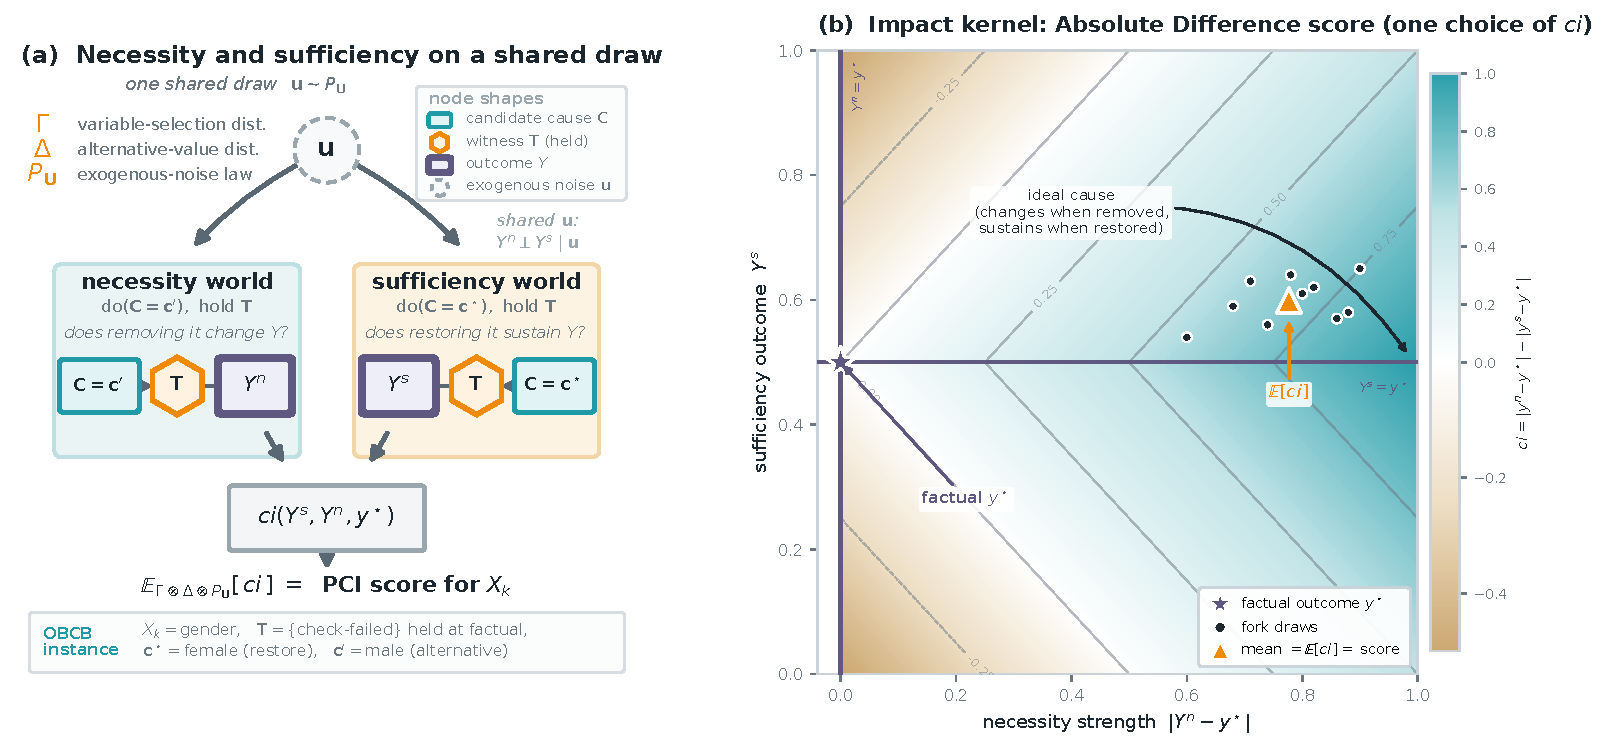
\includegraphics[width=\textwidth]{figures/pci_mechanism.pdf}
\caption{The \ourapproach{} mechanism. \textbf{(a)} For a variable of interest
$X_k$, a single exogenous draw $\mathbf{u}\sim P_{\mathbf{U}}$ together with a
candidate cause set $\mathbf{C}\ni X_k$ and witness set $\mathbf{T}$ from
$\Gamma$ and an alternative value $\mathbf{c}'$ from $\Delta$ defines two
counterfactual worlds on the \emph{same} noise: a \emph{necessity world}
($\mathrm{do}(\mathbf{C}=\mathbf{c}')$, witnesses held) giving $Y^n$, and a
\emph{sufficiency world} ($\mathrm{do}(\mathbf{C}=\mathbf{c}^\star)$, witnesses
held) giving $Y^s$, both drawn against the \emph{same} $(\mathbf{C},\mathbf{T})$
for illustration (the diagonal case of the remark following
Definition~\ref{def:jointnecsuf}). Conditional on $\mathbf{u}$ the two worlds are
independent (the product structure of Definition~\ref{def:jointnecsuf}); the impact
kernel $ci$ scores the pair. \Ourapproach{}'s realised score instead marginalises
$\Gamma$ separately for each world (the independent-product case; see the same
remark) before taking this expectation over $\Delta\otimes P_{\mathbf{U}}$
(Definition~\ref{def:causalimpact}); the two agree here because $ci$ is additively
separable. The strip grounds the schematic in the
OBCB running example. \textbf{(b)} The impact kernel on the \emph{signed} plane
$(Y^n-y^\star,\,Y^s-y^\star)$, shown for the Absolute Difference score
$ci=|y^n-y^\star|-|y^s-y^\star|$, \emph{one} admissible choice of kernel (the
PNS binary score and necessity-only variants are others), before either
deviation is folded by $|\cdot|$. Because $ci$ depends only on the two
absolute deviations, the field is symmetric under an independent sign flip of
either axis: four qualitatively different outcomes, necessity and sufficiency
each landing above or below the factual value, collapse onto the same score
whenever the magnitudes match. The faint cloud is a sample of $(Y^n,Y^s)$
draws (shared with panel~(c)); the four gold points are actual draws, one per
quadrant, with closely matched $|Y^n-y^\star|,|Y^s-y^\star|$, so their nearly
equal $ci$ is a property of the sampled data, not a constructed coincidence.
\textbf{(c)} The same draws' $ci$ values, histogrammed and coloured by sign;
the gold line marks their mean, $\mathbb{E}[ci]$, the \ourapproach{} score for
this variable. This replaces a single scatter-and-mean with the full
distribution the Monte-Carlo estimate is drawn from.}
\label{fig:pci-mechanism}
\end{figure*}

\medskip\noindent Informally, $ci$ is a user-defined scoring rule that translates
the joint sufficiency--necessity measure into a single scalar
(Figure~\ref{fig:pci-mechanism} summarises the whole construction: the two
counterfactual worlds in panel~(a), the kernel that scores them in panel~(b),
and the resulting score as a summary of many such draws in panel~(c)). The
choice is not arbitrary:
the Absolute Difference example below is an instance of L$_1$ distance between outcomes, the
same metric underlying Average Treatment Effect,
 Conditional Average Treatment Effect, and SHAP.
The binary indicator score recovers this as a special
 case when outcomes are binary:
indicators are L$_1$ on $\{0,1\}$. Practitioners
 with reasons to prefer L$_2$ or another
distance measure may substitute it freely; the framework places 
no restriction on $ci$
beyond measurability.

For the OBCB analysis we instantiate $ci$ as the PNS binary score defined in the
following example, with $y^\star = \varname{loan} = 0$. This is the choice that produces
the values in Table~\ref{tab:pci_decomp}.

\begin{example}[PNS for Binary Outcomes]\label{ex:pns_binary}
Assume the outcome $Y$ is binary with $\dom(Y)=\{0,1\}$, and let $y^\star=1$ denote
the factual outcome. Let $Y^s$ and $Y^n$ denote the sufficiency and necessity
outcome variables. Define the causal impact score
\[
ci(y^s,y^n,y^\star)
=
\mathbb{I}\{y^n\neq y^\star\}\,\mathbb{I}\{y^s=y^\star\}.
\]
Then the expected causal impact reduces to
\[
\mathbb{E}\!\left[ci(Y^s,Y^n,1)\right]
=
\mathbb{P}(Y^n=0,\,Y^s=1),
\]
which conceptually coincides with Pearl's probability of necessity and sufficiency (PNS). The alignment is \emph{exact} when $\mathbf{S} = \{X_k\}$, $\mathbf{W}=\emptyset$, and $\dom(X_k)=\{0,1\}$ where, factually, $x_k^\star=1$.
\end{example}

We now illustrate the full computation for Alice's gender attribution using this $ci$.
With $\mathbf{S}=\{\varname{gender},\varname{credit}\}$,
$\mathbf{W}=\{\varname{check\text{-}failed}\}$, $\Gamma_s$ and $\Gamma_w$ uniform,
$\Delta$ a point mass on the alternative binary value, and $y^\star=\varname{loan}=0$,
the exogenous noise $U_\text{check}$ falls into three regions:
\begin{itemize}
\item $u_1$ (prob.\ 0.2): Alice is checked regardless of gender;
  $\varname{check\text{-}failed}=1$ factually.
\item $u_2$ (prob.\ 0.7): Alice is not checked as female but would be as male;
  $\varname{check\text{-}failed}=0$ factually.
\item $u_3$ (prob.\ 0.1): Alice is not checked regardless of gender.
\end{itemize}
In all regions, restoring Alice's factual values always yields a denial, so
$P_k^s(\{0\}\mid\mathbf{u})=\tfrac{2}{3}$ everywhere (four suspect-containing
$(\mathbf{C},\mathbf{T})$ combinations each with $p^\Gamma(\mathbf{C},\mathbf{T})=\tfrac{1}{3}\cdot\tfrac{1}{2}=\tfrac{1}{6}$,
since $\mathbf{S}\cap\mathbf{W}=\emptyset$ here, rejection is vacuous and
$\Gamma$ is just the product of marginals, each contributing probability~1).
The necessity measure varies.

In $u_1$, the witness holds $\varname{check\text{-}failed}=1$.
The four $(\mathbf{C},\mathbf{T})$ contributions, each weighted $\tfrac{1}{6}$, are:
\begin{itemize}
\item[$\circ$] $\mathbf{C}=\{\varname{gender}\}$, $\mathbf{T}=\emptyset$:
  male, $\varname{check\text{-}failed}=1$ propagates structurally
  $\Rightarrow P(\varname{loan}=1)=0.05$.
\item[$\circ$] $\mathbf{C}=\{\varname{gender}\}$,
  $\mathbf{T}=\{\varname{check\text{-}failed}\}$:
  male, witness holds failure
  $\Rightarrow P(\varname{loan}=1)=0.05$.
\item[$\circ$] $\mathbf{C}=\{\varname{gender},\varname{credit}\}$, $\mathbf{T}=\emptyset$:
  male and good credit, check passes
  $\Rightarrow P(\varname{loan}=1)=1.0$.
\item[$\circ$] $\mathbf{C}=\{\varname{gender},\varname{credit}\}$,
  $\mathbf{T}=\{\varname{check\text{-}failed}\}$:
  male and good credit, but witness holds failure
  $\Rightarrow P(\varname{loan}=1)=0.05$.
\end{itemize}
\[ P_k^n(\{1\}\mid u_1)
   = \tfrac{1}{6}(0.05+0.05+1.0+0.05) \approx 0.192. \]

In $u_2$, the witness holds $\varname{check\text{-}failed}=0$.
The four contributions:
\begin{itemize}
\item[$\circ$] $\mathbf{C}=\{\varname{gender}\}$, $\mathbf{T}=\emptyset$:
  male would be checked; $\varname{check\text{-}failed}=1$ propagates structurally
  $\Rightarrow P(\varname{loan}=1)=0.05$.
\item[$\circ$] $\mathbf{C}=\{\varname{gender}\}$,
  $\mathbf{T}=\{\varname{check\text{-}failed}\}$:
  male, witness holds $\varname{check\text{-}failed}=0$, check passes
  $\Rightarrow P(\varname{loan}=1)=1.0$.
\item[$\circ$] $\mathbf{C}=\{\varname{gender},\varname{credit}\}$, $\mathbf{T}=\emptyset$:
  male and good credit, check passes
  $\Rightarrow P(\varname{loan}=1)=1.0$.
\item[$\circ$] $\mathbf{C}=\{\varname{gender},\varname{credit}\}$,
  $\mathbf{T}=\{\varname{check\text{-}failed}\}$:
  male and good credit, witness holds $0$
  $\Rightarrow P(\varname{loan}=1)=1.0$.
\end{itemize}
\[ P_k^n(\{1\}\mid u_2)
   = \tfrac{1}{6}(0.05+1.0+1.0+1.0) \approx 0.508. \]

In $u_3$, male Alice is also not checked ($\varname{check}=0$ regardless of gender),
so all necessity worlds yield denial: $P_k^n(\{1\}\mid u_3)=0$.

Combining, with $ci(y^s,y^n,y^\star)=\mathbb{I}\{y^n\neq y^\star\}\,\mathbb{I}\{y^s=y^\star\}$
and $y^\star=\varname{loan}=0$:
\begin{align*}
\mathrm{PCI}_{\varname{gender}}(\text{Alice})
  &= \mathbb{E}\!\left[ci(Y^s,Y^n,y^\star)\right]
   = \mathbb{P}(Y^n=1,\,Y^s=0) \\
  &= \sum_u p(u)\,P_k^s(\{0\}\mid u)\,P_k^n(\{1\}\mid u) \\
  &= 0.2\times\tfrac{2}{3}\times 0.192
   + 0.7\times\tfrac{2}{3}\times 0.508
   + 0.1\times 0 \\
  &\approx 0.026 + 0.237 = 0.263.
\end{align*}

Table~\ref{tab:pci_decomp} gives the full results for Alice and Bob under these
parameter choices: Pearl's PN/PS/PNS, PCI without witnesses
($\mathbf{W}=\emptyset$), and PCI with the $\varname{check\text{-}failed}$ witness
active, with the latter further decomposed into its necessity and sufficiency
marginals.

\begin{table}[ht]
\centering
\small
\setlength{\tabcolsep}{4pt}
\begin{tabular}{l c c c c c c c}
\toprule
& \multicolumn{3}{c}{Pearl} & PCI & \multicolumn{3}{c}{PCI ($\mathbf{W}=\{\varname{check\text{-}failed}\}$)} \\
\cmidrule(lr){2-4} \cmidrule(lr){6-8}
Person, Variable & PN & PS & PNS & ($\mathbf{W}=\emptyset$) & Necessity & Sufficiency & Total \\
\midrule
Alice (\varname{gender}) & $0.045$ & $1.000$ & $0.045$ & $0.210$
                          & $0.394$ & $0.667$ & $\mathbf{0.263}$ \\
Alice (\varname{credit}) & $0.180$ & $1.000$ & $0.180$ & $0.240$
                          & $0.298$ & $0.667$ & $\mathbf{0.199}$ \\
Bob   (\varname{gender}) & $0.000$ & ---     & $0.000$ & $0.038$
                          & $0.030$ & $0.637$ & $\mathbf{0.019}$ \\
Bob   (\varname{credit}) & $0.900$ & $0.955$ & $0.860$ & $0.228$
                          & $0.188$ & $0.637$ & $\mathbf{0.119}$ \\
\bottomrule
\end{tabular}
\caption{Per-individual responsibility scores for \varname{gender} and \varname{credit}
on $\varname{loan}=0$ in the stochastic OBCB model. Pearl's PN/PS/PNS, PCI without
witnesses ($\mathbf{W}=\emptyset$), and PCI with the \varname{check\text{-}failed}
witness shown side by side; the rightmost three columns decompose PCI($\mathbf{W}=\{\varname{check\text{-}failed}\}$)
into its necessity and sufficiency marginals (their joint expectation is the bold
total). Here the total happens to equal the product of the two marginals because the
sufficiency measure $P_k^s(\cdot\mid\mathbf{u})$ is constant in $\mathbf{u}$ for both
individuals; in general the joint $P_k^{s,n}$ does not factor into the product of its
marginals. Bob's PS for gender is undefined because the conditioning event
$(\text{female}, \text{bad}, \varname{loan}=1)$ has probability zero in the OBCB model;
the PCI marginals are well-defined throughout, since they integrate over $P_{\mathbf{U}}$
rather than conditioning on the factual outcome.}
\label{tab:pci_decomp}
\end{table}

For Alice, PNS and PCI without witnesses both fail \textbf{D-A-rank} (p.~\pageref{desid}):
they rank \varname{credit} above \varname{gender} (0.180 vs.\ 0.045; 0.240 vs.\ 0.210).
PCI with witnesses reverses this (0.263 vs.\ 0.199), satisfying \textbf{D-A-rank} as well
as \textbf{D-A1} and \textbf{D-A2} (both values positive). Holding
\varname{check\text{-}failed} at its factual value blocks the credit-check bottleneck in
noise realizations where Alice was checked, isolating gender's structural role. The
\varname{check\text{-}failed} witness is the decisive ingredient.

For Bob, \textbf{D-B2} and \textbf{D-B-rank} hold under all three methods:
\varname{credit} is ranked above \varname{gender} throughout. \textbf{D-B1} requires
strictly positive attribution for \varname{gender}: PNS returns exactly 0.000 and
therefore fails, because $P(\varname{loan}=1\mid\varname{gender}=\text{female},
\varname{credit}=\text{bad})=0$ makes the counterfactual necessity calculation zero,
missing gender's indirect role in opening the credit evaluation. PCI with witnesses
returns 0.019, correctly capturing this indirect contribution. The cross-individual
desideratum \textbf{D-comp} holds under both PCI (0.263 $>$ 0.019) and PNS
(0.045 $>$ 0.000). A full verification of all seven desiderata is given at the end
of this section.

The PNS and PCI (no witnesses) columns differ even though neither uses witnesses,
because PCI still $\Gamma$-averages over candidate suspect sets.  With
$|\mathbf{S}|=2$ PCI averages over $\{\varname{gender}\}$, $\{\varname{credit}\}$,
and $\{\varname{gender},\varname{credit}\}$ (each weighted $\tfrac{1}{3}$),
whereas PNS evaluates a single counterfactual on one variable at a time.
Property~(i) below establishes that the two agree exactly when $|\mathbf{S}|=1$
(single suspect, no witnesses, binary outcome), whereas the OBCB setup uses
$|\mathbf{S}|=2$ deliberately, to demonstrate joint-subset attribution.

% \begin{definition}[Causal impact and its push-forward]
% Let $y^s$ denote the outcome in the \emph{sufficiency world}, $y^n$ denote the outcome in the \emph{necessity world}, and $y^\star$ the outcome in the factual world. By construction, these are independent conditional on $\mathbf{u}$, and so we get the joint:
% \begin{align}
%  p(\langle y^s, y^n \rangle \mid \mathbf{u})  & = p^s_k(y^s \mid \mathbf{u}) \; {p}^n_k(y^n \mid \mathbf{u}).
% \end{align}

% \noindent which also generates a push-forward on any causal impact scoring function $ci(y^s, y^n, y^\star)$, whose expectation is a summary of causal impact.
% \begin{align}\label{eq:score}
% \mathbb{E}_{\mathbf{u}}\Big[\, \mathbb{E}_{y^s, y^n \mid \mathbf{u}} \big[ ci(y^s, y^n, y^\star) \big] \,\Big]
% =\\ \iiint  ci(y^s, y^n, y^\star) \; p^s_k(y^s \mid \mathbf{u}) \; p^n_k(y^n \mid \mathbf{u}) p(\mathbf{u}) 
%    \, dy^s \, dy^n \, d\mathbf{u}. \nonumber
% \end{align}
% \end{definition}

% With this in place, we can characterize a number of causal impact measures by first defining a \emph{causal impact function} as the expectation of a causal impact function taken with respect to the joint measure on factual and counterfactual outcomes.

\subsection{Continuous Outcomes and the General Causal Impact Function}
\label{sub:continuous_ci}

\noindent The causal impact function $ci$ is a user-defined component of \ourapproach, and different choices encode different causal questions. In the benchmarking experiments of \cref{sec:ac_benchmark}, we instantiate $ci$ using only the necessity component, since Halpern’s actual causality has no sufficiency counterpart: necessity-only attribution allows a direct parallel comparison. The full framework incorporating both $Y^s$ and $Y^n$ is instantiated in the PNS binary
example above and in the Absolute Difference example below; the OBCB analysis of this
section (Tables~\ref{tab:pci_decomp}--\ref{tab:desiderata}) provides a concrete
validation, since the PNS binary $ci$ jointly conditions on $Y^s=y^\star$ and
$Y^n\neq y^\star$ and it is precisely this combination that produces the correct
\textbf{D-A-rank} ordering. Further experiments using the full $ci$ on continuous outcomes are presented in
the signal-with-mediation example (Section~\ref{sec:signal}), the synthetic
evaluation (\cref{sub:synthetic}), and the SIR benchmark
(\cref{sec:sir_benchmark}).

When the outcome variable $Y$ is continuous rather than binary, indicators are replaced by a distance-based score that measures how far the necessity and sufficiency worlds land from the factual value $y^\star$.
The natural choice, paralleling L$_1$-based scores such as ATE and SHAP, is the absolute difference.

\begin{example}[Absolute Difference Impact Score] \label{ex:absolute_score}
We can develop an analogous measure for continuous outcomes where we increase attribution with distance from the factual value $y^\star$ in the necessity world and decrease impact with distance to the factual value in the sufficiency world.
\begin{align*}
ci(y^s, y^n, y^\star) & = \vert y^n - y^\star \vert   - \vert y^s - y^\star \vert.
\end{align*}
\end{example}

\noindent Two one-sided instances of this score recur in the experiments: a
necessity-only $ci_N$ and a sufficiency-only $ci_S$ (\cref{sub:synthetic}), whose sum
returns the absolute-difference $ci$ above. Each is a choice of $ci$ in the sense of
Definition~\ref{def:causalimpact}.

With the full machinery in place (structural model, variable selection, alternative
value distribution, joint necessity-sufficiency measure, and causal impact function),
\ourapproach delivers the following properties.
\begin{enumerate}[label=(\roman*)]
\item \textbf{Generalisation of PN/PS/PNS.} When $\mathbf{S}=\{X_k\}$,
  $\mathbf{W}=\emptyset$, and $\dom(X_k)=\{0,1\}$, the PNS binary $ci$ recovers Pearl's
  probability of necessity and sufficiency exactly; PN and PS are recovered by the
  corresponding one-sided $ci$ choices.
\item \textbf{Connection to actual causality.} For suitable $\Gamma$
  and $\Delta$, \ourapproach recovers Halpern's actual causality judgements
  (Section~\ref{sec:relation_with_ac}).
\item \textbf{Necessity--sufficiency decomposition.} $P_k^s$ and $P_k^n$ are defined and
  interpretable independently; practitioners may choose a $ci$ that uses either alone
  or both, depending on whether the causal question concerns necessity, sufficiency,
  or both.
\item \textbf{Witness-mediated symmetry breaking.} Holding intermediate variables fixed
  via $\mathbf{W}$ disambiguates overdetermination and undercutting scenarios where
  necessity-only methods assign equal or zero attribution, as demonstrated above for
  Alice and Bob, and further developed in Section~\ref{sec:shap_examples} (SHAP and
  Causal SHAP comparison), \cref{sub:synthetic} (synthetic overdetermination
  and undercutting archetypes), and \cref{sec:ac_benchmark} (witness ablation
  on the scaled throwing problem).
\item \textbf{Composability.} $\Gamma$, $\Delta$, and $ci$ are probability distributions
  and a measurable function respectively; they slot naturally into Bayesian pipelines,
  accept posteriors as inputs, and admit Monte Carlo estimation without modification to
  the core formalism.
\end{enumerate}

\subsection{Back to the Running Example: Verifying the Desiderata}
\label{sub:verify_desiderata}

Table~\ref{tab:desiderata} verifies the seven desiderata introduced at the start of this
section (p.~\pageref{desid}) against the values in Table~\ref{tab:pci_decomp}.
PCI with witnesses satisfies all seven; PCI without witnesses fails \textbf{D-A-rank};
PNS fails \textbf{D-A-rank} and \textbf{D-B1}.
(The table uses the shorthand $|R(V\mid\text{person})|$ for
$|R(V\rightsquigarrow\varname{loan}\mid\text{person})|$.)

\begin{table}[ht]
\centering
\resizebox{\linewidth}{!}{%
\begin{tabular}{lccc}
\toprule
Desideratum & PNS & PCI (no wit.) & PCI (with wit.) \\
\midrule
\textbf{D-A1}: $|R(\varname{gender}\mid\text{Alice})| > 0$
  & $\checkmark$\ 0.045 & $\checkmark$\ 0.210 & $\checkmark$\ 0.263 \\
\textbf{D-A2}: $|R(\varname{credit}\mid\text{Alice})| > 0$
  & $\checkmark$\ 0.180 & $\checkmark$\ 0.240 & $\checkmark$\ 0.199 \\
\textbf{D-A-rank}: $|R(\varname{gender}\mid\text{Alice})| > |R(\varname{credit}\mid\text{Alice})|$
  & $\times$\ $0.045 {<} 0.180$
  & $\times$\ $0.210 {<} 0.240$
  & $\checkmark$\ $0.263 {>} 0.199$ \\
\textbf{D-B1}: $|R(\varname{gender}\mid\text{Bob})| > 0$
  & $\times$\ 0.000 & $\checkmark$\ 0.038 & $\checkmark$\ 0.019 \\
\textbf{D-B2}: $|R(\varname{credit}\mid\text{Bob})| > 0$
  & $\checkmark$\ 0.860 & $\checkmark$\ 0.228 & $\checkmark$\ 0.119 \\
\textbf{D-B-rank}: $|R(\varname{credit}\mid\text{Bob})| > |R(\varname{gender}\mid\text{Bob})|$
  & $\checkmark$\ $0.860 {>} 0.000$
  & $\checkmark$\ $0.228 {>} 0.038$
  & $\checkmark$\ $0.119 {>} 0.019$ \\
\textbf{D-comp}: $|R(\varname{gender}\mid\text{Alice})| > |R(\varname{gender}\mid\text{Bob})|$
  & $\checkmark$\ $0.045 {>} 0.000$
  & $\checkmark$\ $0.210 {>} 0.038$
  & $\checkmark$\ $0.263 {>} 0.019$ \\
\bottomrule
\end{tabular}}
\caption{Verification of the seven desiderata (p.~\pageref{desid}) against the values in
Table~\ref{tab:pci_decomp}. PCI with witnesses satisfies all seven; PCI without witnesses
fails \textbf{D-A-rank}; PNS fails \textbf{D-A-rank} and \textbf{D-B1}.}
\label{tab:desiderata}
\end{table}

\medskip\noindent\textit{PNS fails \textbf{D-A-rank} and \textbf{D-B1}. The D-A-rank
failure reflects that without a \varname{check\text{-}failed} witness,
necessity-based attribution cannot distinguish Alice's gender (which blocked the
evaluation entirely) from her credit (which would only have mattered had she been
evaluated). The D-B1 failure reflects that PNS assigns Bob's gender exactly zero:
because $P(\varname{loan}=1\mid\text{female},\text{bad})=0$,
the counterfactual necessity calculation returns zero, missing gender's indirect role in
opening the credit evaluation. The \varname{check\text{-}failed} witness resolves both.}

To close this section, it is worth comparing PCI's decomposition with the one already
present in Pearl's framework. Pearl's framework defines three related but distinct
binary scores: the probability of necessity
$\mathrm{PN} = P(Y_{x'} = y' \mid X = x^\star, Y = y^\star)$, the probability of sufficiency
$\mathrm{PS} = P(Y_{x^\star} = y^\star \mid X = x', Y = y')$, and their joint
$\mathrm{PNS} = P(Y_{x^\star} = y^\star, Y_{x'} = y')$. The first two are conditional
probabilities; $\mathrm{PNS}$ is unconditional, and the three satisfy
$\mathrm{PNS} = \mathrm{PN}\cdot P(Y_{x^\star}=y^\star) = \mathrm{PS}\cdot P(Y_{x'}=y')$ rather
than $\mathrm{PNS} = \mathrm{PN}\cdot\mathrm{PS}$ (which would require
$Y_{x^\star}\perp Y_{x'}$, an assumption typically violated since the two potential
outcomes share exogenous noise). PCI admits a related split: with
$ci = \mathbb{I}\{y^n \neq y^\star\}\,\mathbb{I}\{y^s = y^\star\}$,
\[
\mathbb{E}[ci(Y^s, Y^n, y^\star)]
= \int P^s_k(\{y^\star\}\mid\mathbf{u})\,P^n_k(\{1{-}y^\star\}\mid\mathbf{u})\,dP_{\mathbf{U}},
\]
giving a \emph{sufficiency marginal} and a \emph{necessity marginal} that record how
often, on average, restoring the factual values of a suspect set containing $X_k$
reproduces the factual outcome, and how often substituting alternatives overturns it.
The two marginals are independent given $\mathbf{u}$.

The components are not identical to Pearl's: $\mathrm{PN}$ and $\mathrm{PS}$ condition
on the factual outcome and consider a single counterfactual flip; PCI's marginals
integrate over $P_{\mathbf{U}}$, average over suspect sets weighted by $\Gamma$, and
hold the witness configurations fixed when active. Table~\ref{tab:pci_decomp} (presented
earlier) places both decompositions side by side for \varname{gender} and
\varname{credit}.


For Alice's gender, $\mathrm{PN} = 0.045$ is the bare probability that a male with bad
credit would have been approved; PCI's necessity marginal is $0.394$, nearly an order of
magnitude higher, because the \varname{check\text{-}failed} witness keeps the
credit-check bottleneck active when the male counterfactual would otherwise have been
checked and might still have failed, structural information that the unconditional
$\mathrm{PN}$ cannot register. For Bob's gender, $\mathrm{PN}$ is exactly $0$ (a female
with bad credit cannot be approved in this model) and $\mathrm{PS}$ is undefined; PCI's
marginals remain well-defined at $0.030$ and $0.637$, recovering the indirect role of
gender in opening the evaluation.

The next section turns from comparing PCI with Pearl's family of counterfactual scores
to comparing it with the SHAP family, methods grounded in cooperative game theory
rather than in structural counterfactual reasoning.
Section~\ref{sec:shap_examples} re-runs the OBCB analysis under plain and Causal
SHAP, then introduces a continuous mediation example where the two SHAP variants
diverge from each other and from PCI, with explicit desiderata recorded throughout.

